%!TEX root = ../thesis.tex
% **************************** Define Graphics Path **************************
\ifpdf
\graphicspath{{Chapter4/Figs/Raster/}{Chapter4/Figs/PDF/}{Chapter4/Figs/}}
\else
\graphicspath{{Chapter4/Figs/Vector/}{Chapter4/Figs/}}
\fi


%*******************************************************************************
%****************************** Fourth Chapter *********************************
%*******************************************************************************

\chapter{Methodology}
\label{chapter4}
This chapter presents the computational method developed in this thesis. We start by introducing each component of the method separately before presenting how they fit together into a single procedure. We discuss neural networks, automatic differentiation, gradient estimation, gradient-based optimisation, as well as importance sampling. Finally, we present the actual implementation in \emph{JAX}, and discuss computational considerations and intricacies of thereof.

\section{Neural Networks} % ~150 words
\subsection{The Multilayer Perceptron}
The \textbf{multilayer perceptron} (MLP), also referred to as a \textbf{deep feedforward network} or simply a \textbf{deep neural network} (DNN), is the paradigmatic model of deep learning and serves as a foundation of more advanced models. In essence it is nothing more than a mapping of inputs to outputs
\begin{equation}
	f(\mathbf{x}; ~\theta): \mathbb{R}^\text{in} \rightarrow \mathbb{R}^{\text{out}},
\end{equation}
which is structured in a certain way and depends on parameters $\theta$. The mapping is a composition of vector-valued functions $f$ which are called \emph{layers} of the network, and with each layer we associate variational parameters $\mathbf{w}$, or simply the weights. The MLP can be described with a directed acyclic graph which details the compositions of the layers. The simplest and most common is a chain of compositions, Fig~\ref{fig:mlp}b, 
\begin{equation}
f_{\text{MLP}} = \left(f^{(n)} \circ f^{(n-1)} \circ \cdots \circ f^{(2)} \circ f^{(1)} \right)(\mathbf{x}),
\end{equation}
where the input $\textbf{x}$ passes through \emph{hidden layers} before the \emph{output layer} outputs the result. The length of this chain is the \emph{depth} of the network, and the dimensionality of hidden layers is the \emph{width} of the network. We can interpret each transformation $f^{(i)}$ as consisting of a unit/node/neuron for each input dimension, which is vector-to-scalar transformation, Fig~\ref{fig:mlp}a.
\begin{figure}[H]
	\centering
	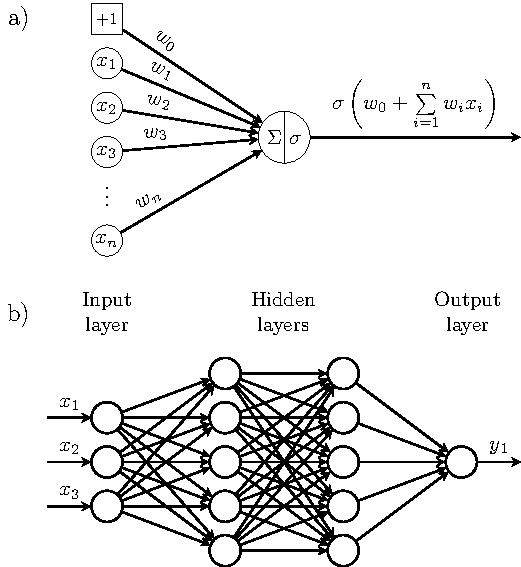
\includegraphics[width=\linewidth]{Chapter4/Figs/Vector/mlp.pdf}
	\caption[Multilayer Perceptron]{\textbf{Multilayer Perceptron.} \textbf{top: }A node outputs the activation function $\sigma$ evaluated at the weighted average over outputs from the previous layer and bias. \textbf{bottom: } A MLP with two hidden layers ($f^{(1)}: \mathbb{R}^3 \rightarrow \mathbb{R}^4$, $f^{(2)}: \mathbb{R}^4 \rightarrow \mathbb{R}^4$, $f^{(3)}: \mathbb{R}^4 \rightarrow \mathbb{R}$).}
	\label{fig:mlp}
\end{figure} 
\noindent
The simplest layer would be a linear one, composed of
\begin{equation}
f(\mathbf{x}; \mathbf{w}, b) = \mathbf{x}^\intercal \mathbf{w} + b.
\end{equation}
However, a linear neural network famously cannot learn the XOR function~\cite{minsky2017perceptrons}, and in practice a nonlinearity or \emph{activation} function $g(\cdot)$ is used in each node to bolster the network's representational power
\begin{equation}
f(\mathbf{x}; \mathbf{w}, b) = g\left(\mathbf{x}^\intercal \mathbf{w} + b\right).
\end{equation}
A variety of activations have been used, namely $\tanh(\cdot)$ and the logistic sigmoid $\sigma(\cdot)$, but have since been displaced by the use of the \textbf{rectified linear unit} or $\operatorname{ReLu}(\cdot)$, which is advantageous for training, for the output layer we will use the \emph{softplus}, which fulfils the requirement of being positive everywhere, Fig.~\ref{fig:activations}. A multilayer perceptron is a \textbf{universal function approximator}, meaning that with at least one hidden layer it can approximate any Borel measurable function mapping from a finite-dimensional space to another with desired accuracy, given sufficient hidden units~\cite{leshno1993multilayer}. This means that a large enough network will be able do represent the rates, however this provides no guarantee that learning the correct rates will be efficient or possible. 
\begin{figure}[H]
	\centering
	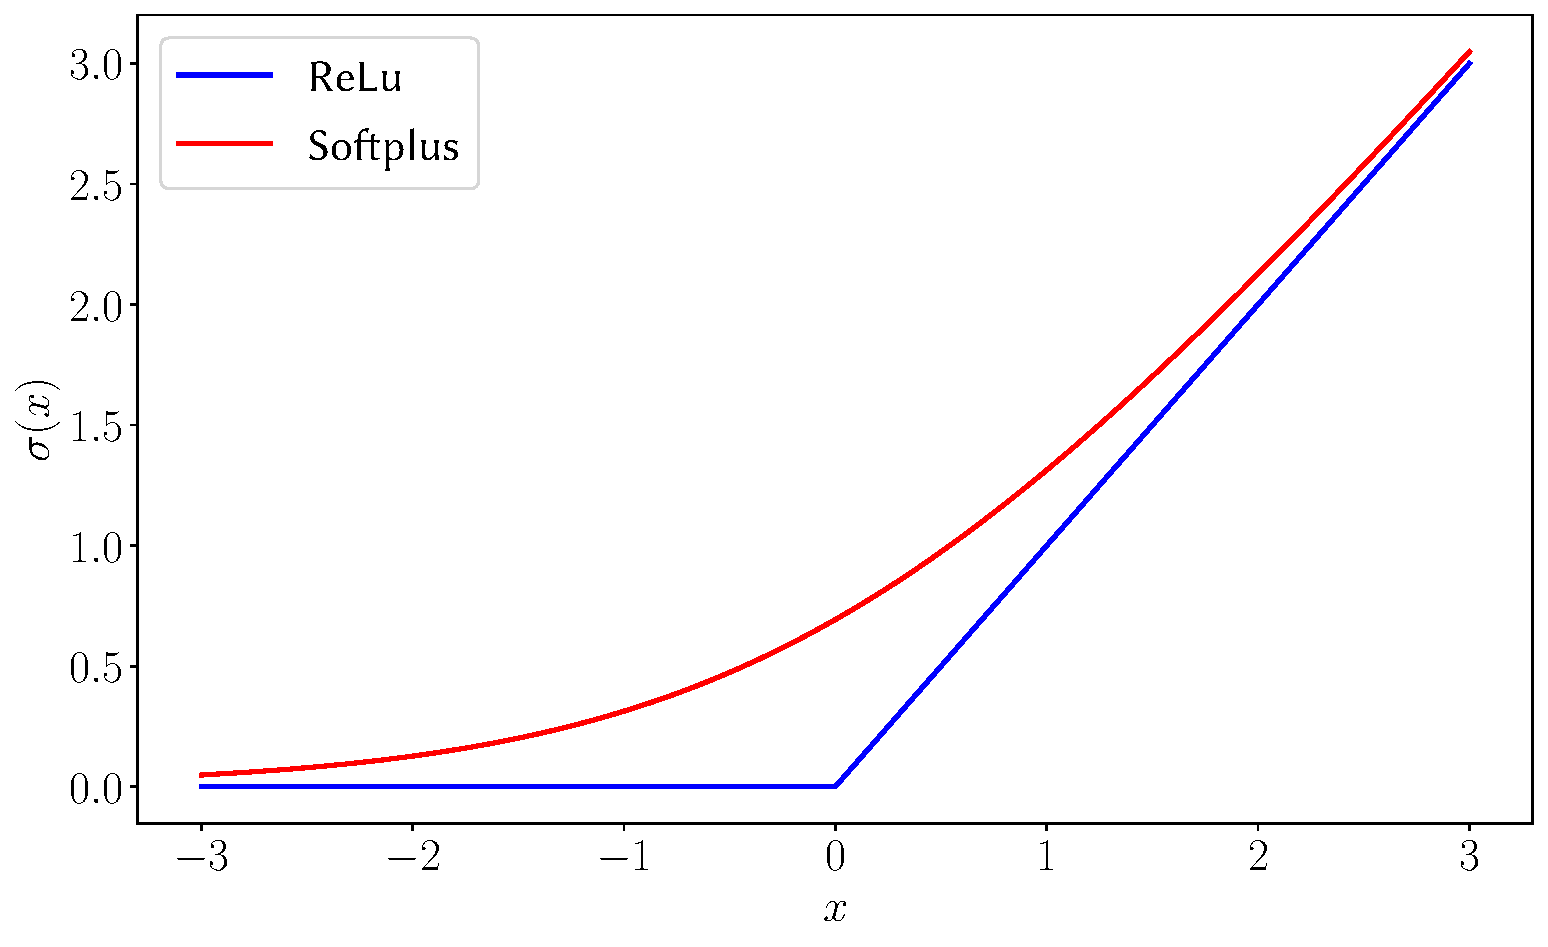
\includegraphics[width=0.7\linewidth]{Chapter4/Figs/Vector/activations}
	\caption[Activation functions]{\textbf{Activation functions.} $\operatorname{ReLu}$ and Softmax nonlinearities.}
	\label{fig:activations}
\end{figure}

\subsection{Convolutional Neural Networks} % saturday morning
\label{subsec:nn-cnn} 
Convolutional neural networks (CNN)~\cite{lecun1989generalization} are neural network architectures specialised to work with grid/image inputs. They make use of three powerful concepts to increase performance, \textbf{sparse interactions}, \textbf{parameter sharing} and \textbf{equivariant representations}~\cite{goodfellow2016deep}. At the core of a CNN is the \emph{convolutional} layer in which the input $I$ is convolved with the \emph{kernel} $K$ as 
\begin{equation}
	\label{eq:convolution}
	S_{i,j} = (I * K)_{i,j} = \sum_m \sum_n I_{m,n} K_{i-m, j-n},
\end{equation}
in two dimensions, Fig.~\ref{fig:pcnn}a. Outputs of convolutions are referred to as \emph{feature maps}. In practice the kernel $K$ is much smaller than the input, meaning that each neuron is connected only to a small fraction of neurons in the previous layer, hence the layers are sparsely connected in contrast to the fully connected layer Fig.~\ref{fig:pcnn}c. This decreases the number of weights and operations required. Moreover, the kernel is applied everywhere in the input, meaning the weights are shared across all connections and need to be learned for the whole input as opposed to every single position in the input. This makes the convolutional layer much more memory efficient than the fully connected layer. Moreover, the nature of convolution in eq.~\eqref{eq:convolution} means that the convolutional layer is equivariant to translation, i.e. a translation of the input results in the same translation of the output. Altogether, a convolutional layer is a transformation acting on a batch of examples $N_b$ with channels $N_c$
\begin{equation}
	f: \mathbb{R}^{(N_b, N_w, N_h, N_c)} \rightarrow \mathbb{R}^{(N_b, O_w, O_h, N_c)}.
\end{equation}
The output dimensions also depend on the \emph{stride} (how quick the kernel travels)~$N_S$ and \emph{padding}~$N_P$ (how much the dimension of input is increased), Fig.~\ref{fig:pcnn}a,
\begin{equation}
	O_{\text{out}} = \frac{N_{\text{in}}-N_K+2N_P}{N_S}+1.
\end{equation}
Alongside convolutional layers CNNs often employ \emph{pooling} layers which downsample the input by combining a cluster of neurons into a single one. \emph{Max} and \emph{average} pooling are in common use, the pooling output is the max or average of the cluster respectively. A pooling layer can act globally, on the whole feature map, or locally. 

The models we are interested in will be image-to-image networks that preserve the input shape, as the outputs will represent the rates corresponding to adjacent states. In the Ising model, the output at $(i, j)$ is the rate associated with transition $s \rightarrow s^\prime$ where the spin at $(i, j)$ is flipped.
\subsubsection{Periodic CNN}
The simplest model we will use is a CNN in which all layers preserve the shape of the input $N_\text{in} = O_\text{out}$. This means that the input into each layer needs to be padded
\begin{equation}
		N_{P} = \frac{N_{K}-1}{2},
\end{equation}
for $N_S = 1$. Given that the underlying lattice is chosen to be periodic, we use periodic instead of zero padding, see Fig.~\ref{fig:pcnn}b. Hidden units use $\operatorname{ReLu}$ and the last layer uses $\operatorname{softmax}$. 
\begin{figure}[H]
	\centering
	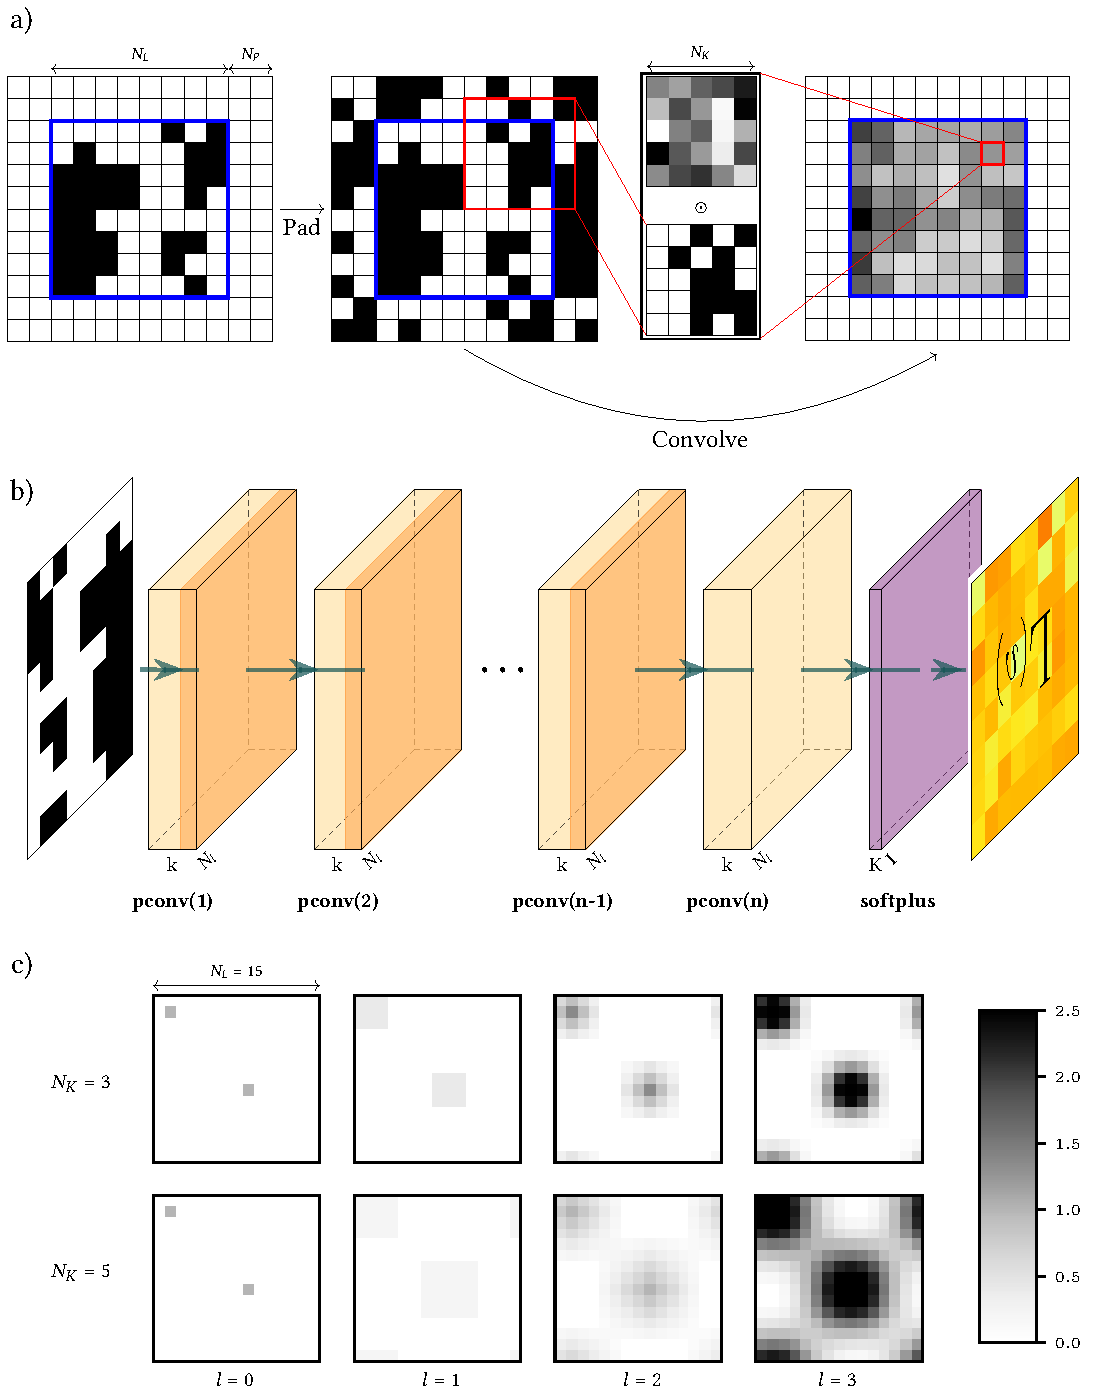
\includegraphics[width=\linewidth]{../diagrams/pcnn/pcnn}
	\caption[Periodic CNN]{\textbf{Periodic CNN} \textbf{top:} Each layer consists of periodic padding, and then convolving. The output shape matches the input shape. \textbf{middle:} The pCNN architecture, takes state $s$ as input and outputs rates $\Gamma(s)$, similar to~\cite{gispen2020ground}. \textbf{bottom: } While the receptive field of a single node is reduced in a CNN, faraway nodes are still connected indirectly after enough layers, how many layers depends on the kernel size and stride. Figure shows successive applications of the convolutional layers for $N_s=1$ and $N_K = 3$ or $N_K=5$. }
	\label{fig:pcnn}
\end{figure}
\subsection{Group-Equivariant CNN}
The basic convolutional layer is translation equivariant, providing an advantage when we expect the same equivariant behaviour between the input and output. Alongside translational symmetry we can take advantage of other symmetries present in the lattice model. Recent work~\cite{cohen2016group, bronstein2021geometric} in the field of \textbf{geometric deep learning} has shown how to construct layers equivariant to arbitrary group symmetry, in the case of discrete grid-like data referred to as \textbf{group-equivariant} convolutional layers. At the core of \emph{group convolution} is moving the filter using group action (rotation, translation, etc.). Adopting notation of Bronstein~\cite{bronstein2021geometric}, we write a group convolution as the inner product of the input $x$ and a filter transformed by group element $\mathfrak{g} \in \mathfrak{G}$ via group representation $\rho(\mathfrak{g})$ as $\rho(\mathfrak{g}) \theta_{u}=\theta_{\mathfrak{g}^{-1} u}$,
\begin{equation}
(x \star \theta)(\mathfrak{g})=\sum_{u \in \Omega} x_{u} \rho(\mathfrak{g}) \theta_{u}.
\end{equation}
\begin{figure}[h]
	\centering
	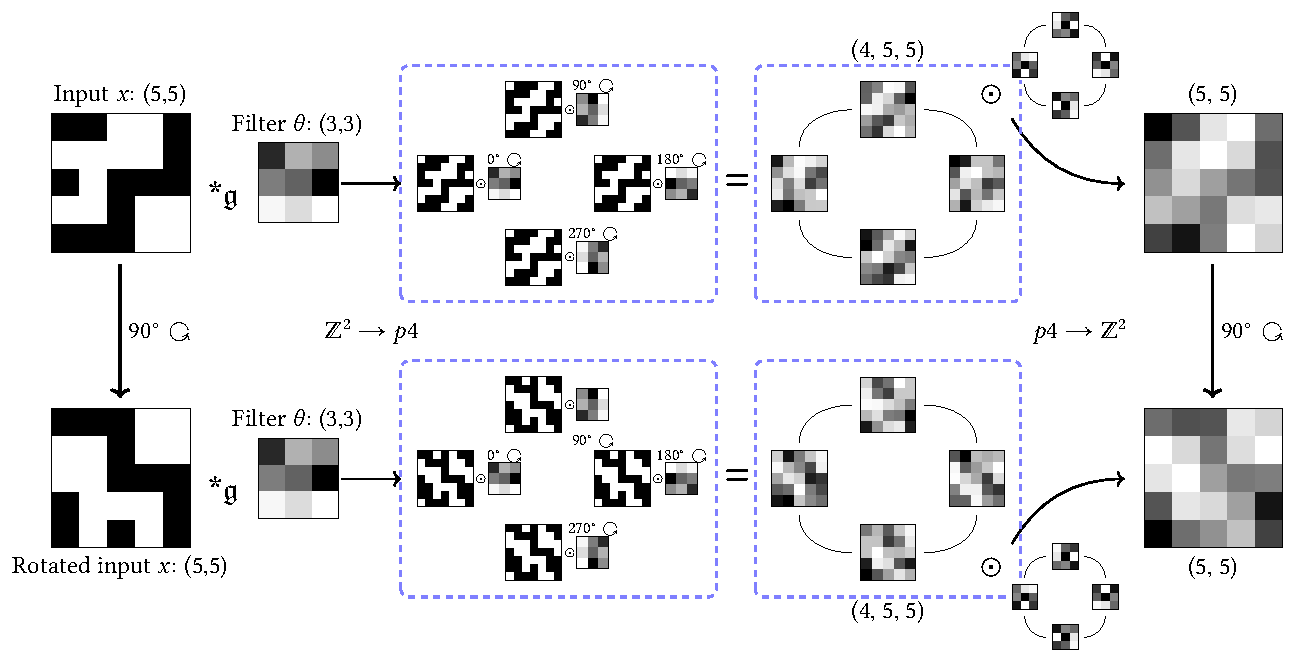
\includegraphics[width=\linewidth]{Chapter4/Figs/Vector/gcnn}
	\caption[Group-equivariant convolution]{\textbf{g-CNN layer.} Comparison of rotated inputs passing through two $p4$ equivariant layers. The first layer $\mathbb{Z}^2 \rightarrow p4$ produces a structured output, one convolution per each rotation of the filter $\theta$, the second layer $p4 \rightarrow \mathbb{Z}^2$ is an elementwise convolution between the structured output and rotations of the second filter. The layers are equivariant to $\frac{\pi}{2}$ rotation.}
	\label{fig:gcnn}
\end{figure}
We can separate the ordinary convolution from additional group transformations by writing a general group element $\mathfrak{g} \in \mathfrak{G}$ as a composition of a translation $\mathfrak{t}$ and rotation $\mathfrak{r}$, $\mathfrak g = \mathfrak{tr}$, and using  $\rho(\mathfrak{t r})=\rho(\mathfrak{t}) \rho(\mathfrak{r})$
\begin{equation}
	(x \star \theta)(\mathfrak{t r}) =\sum_{u \in \Omega} x_{u} \rho(\mathfrak{t}) \rho(\mathfrak{r}) \theta_{u} =\sum_{u \in \Omega} x_{u}(\rho(\mathfrak{r}) \theta)_{u-\mathfrak{t}},
\end{equation}
This yields a standard convolution with a transformed filter $\rho(\mathfrak{r})\theta$, meaning that we can implement the group-equivariant layer by first transforming the filter and performing convolution with each of these transformations, for details see Fig.~\ref{fig:gcnn} and~\cite{cohen2016group}.

\section{Gradient-based optimisation}
\label{sec:gbopt}
There are three components needed to perform gradient based optimisation. \textbf{Automatic differentiation} (AD), the ability to efficiently and reliably differentiate through computations. \textbf{Gradient estimation} methods for estimating gradients of expectations of functions, and an \textbf{optimisation algorithm}.

\subsection{Automatic differentiation}
\label{subsec:autodiff}
The demand for automatic evaluation of derivatives is today greater than ever, and automatic differentiation has seen wide adoption within the scientific computing and machine learning communities~\cite{lyu2013automatic, tamayo2018automatic, baydin2018automatic}, with the development of high profile libraries such as \emph{PyTorch}~\cite{paszke2017automatic}, \emph{TensorFlow}~\cite{abadi2016tensorflow}, or \emph{JAX}~\cite{jax2018github}. Not to be confused with numerical or symbolic differentiation, \textbf{automatic differentiation} provides a way to mechanically find derivatives of functions expressed as a computer program, with certain complexity guarantees~\cite{barak2016history}. While modern implementations employ a variety of tricks, AD has two basic \emph{modi operandi} of calculating partial derivatives of $f(x_1, x_2, \ldots, x_n): \mathbb{R}^n \rightarrow \mathbb{R}^m$ at $\mathbf{a}$. We start by representing the computation $y = f(\mathbf{x})$ as an \emph{evaluation trace} of elementary operations, composed of inputs, intermediate values, and outputs:
\begin{itemize}
	\item \textbf{Forward accumulation mode}~\cite{wengert1964simple}:  In forward mode, when evaluating the partial derivative w.r.t $x_j$, we associate each intermediate value $v_i$ with the partial derivative $\frac{\partial v_i}{\partial x_j}$. We then apply the chain rule to each operation in the evaluation trace, producing the derivative trace. A single forward pass, in tandem passing both primals $v_i$ and their tangents $\frac{\partial v_i}{\partial x_j}$ through the trace, produces the output of the function, as well as the desired partial derivative. Forward mode AD produces one \emph{column} of the Jacobian $\textbf{J}_f$ at each pass, and is suited for functions with $n \ll m$.
	
	\item \textbf{Reverse accumulation mode}~\cite{speelpenning1980compiling}:
\end{itemize}
AD is most commonly implemented in one of two ways, either by \emph{operator overloading}, abstracting away the derivative part of the calculation, e.g. in \emph{TensorFlow} of \emph{JAX}~\cite{abadi2016tensorflow, jax2018github}. Or alternatively via \emph{source code transformation}, where a new function is constructed by altering the source code, see \emph{Zygote}~\cite{innes2018don}.

\subsection{Gradient estimation}
\label{subsec:gbopt-gest}
The problem of stochastic gradient estimation of an expectation of a function is a well studied problem that transcends machine learning and has a variety of applications~\cite{chriss1997black, schrittwieser2020mastering}. Different estimators differ in from and their properties, variance being one of the most important. In their review~\cite{mohamed2020monte} Mohamed et al. categorise MC gradient estimators into three categories

\subsubsection{Score-function estimator}
\emph{Score-function estimator}: The score function is a logarithm of a probability distribution w.r.t to distributional parameters. It can be used as a gradient estimator
\begin{equation}
\begin{aligned}
\nabla_{\boldsymbol{\theta}} \mathbb{E}_{p_{\boldsymbol{\theta}}(\mathbf{x})}[f(\mathbf{x})] &=  \nabla_{\boldsymbol{\theta}} \int p_{\boldsymbol{\theta}}(\mathbf{x}) f(\mathbf{x}) d \mathbf{x} \\
&= \mathbb{E}_{p_{\boldsymbol{\theta}}(\mathbf{x})}\left[f(\mathbf{x}) \nabla_{\boldsymbol{\theta}} \log p_{\boldsymbol{\theta}}(\mathbf{x})\right].
\end{aligned}
\end{equation}
The score-function estimator is compatible with any cost function, it requires that the measure $p_{\boldsymbol{\theta}}(\mathbf{x})$ is differentiable and easy to sample. Importantly it is applicable to both discrete and continuous distribution, but has the drawback of having high variance.

\subsubsection{Pathwise estimator}
Continuous distributions can be sampled either directly by generating samples from the distribution $p_{\boldsymbol{\theta}}(\mathbf{x})$ or indirectly, by sampling from a simpler base distribution $p(\boldsymbol{\epsilon})$ and transforming the variate through a deterministic path $g_{\boldsymbol{\theta}}(\boldsymbol{\epsilon})$. Using this, it is possible to move the source of randomness in such a way that the objective is differentiable. In essence this approach pushes the parameters of the measure into the cost function which is then differentiated. The estimator is
\begin{equation}
\begin{aligned}
\nabla_{\boldsymbol{\theta}} \mathbb{E}_{p_{\boldsymbol{\theta}}(\mathbf{x})}[f(\mathbf{x})] 
&=\nabla_{\boldsymbol{\theta}} \int p_{\boldsymbol{\theta}}(\mathbf{x}) f(\mathbf{x}) d \mathbf{x} \\
&= \nabla_{\boldsymbol{\theta}} \int p(\boldsymbol{\epsilon}) f(g_{\boldsymbol{\theta}}(\boldsymbol{\epsilon})) d \boldsymbol{\epsilon} \\
&= \mathbb{E}_{p(\boldsymbol{\epsilon})}\left[\nabla_{\boldsymbol{\theta}} f(g_{\boldsymbol{\theta}}(\boldsymbol{\epsilon}))\right].
\end{aligned}
\end{equation}
\begin{figure}
	\centering
	\subfloat[Original]{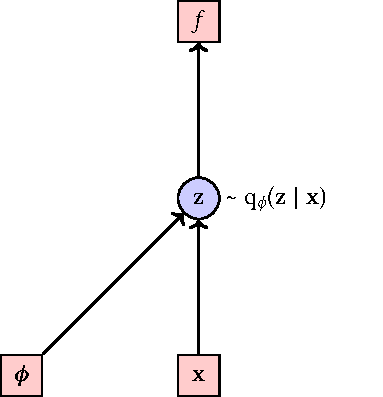
\includegraphics[height=5cm]{Appendix2/Figs/Vector/reparam_diagram.pdf}}
	\quad
	\subfloat[Reparametrized]{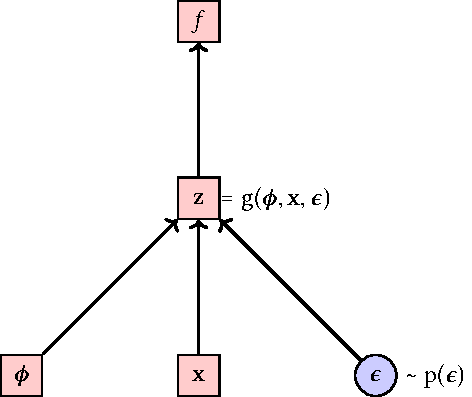
\includegraphics[height=5cm]{Appendix2/Figs/Vector/reparam_diagram2.pdf}}
	\caption[The reparametrization trick]{\textbf{The reparametrization trick}, adapted from~\cite{kingma2017variational}. Stochasticity of the $\mathbf{z}$ node is pushed out into a separate input to the same node, resulting in deterministic gradients w.r.t $\boldsymbol{\phi}$ through the node.}
	\label{fig:reparam}
\end{figure}
This was the gradient estimator originally used in the VAE implementation~\cite{kingma2013auto} there named as the \emph{reparametrization trick}, see also Figure~\ref{fig:reparam}. In many cases the transformation paths are so simple they can be implemented in one line of code, referred to as \emph{one-liners}. The pathwise-estimator can only be used on differentiable cost functions, but is easy to implement and crucially has lower variance than the score-function estimator.

\subsubsection{Measure-valued gradient estimator}
Which exploits the properties of signed-measures, is beyond the scope of this report.

\begin{enumerate}
	\item measure-valued
	\item how does this apply to our objective?
\end{enumerate}

\subsection{Optimisation algorithms}

\section{Monte Carlo Importance Sampling}
\label{sec:Impl-MCIP}
The most common application of Monte Carlo methods is evaluation of integrals in high dimensional space. There MC has a distinct advantage over quadrature methods, as the statistical error decreases with the square root of samples irregardless of the dimensionality of the problem. Integrals of a function $g(\mathbf{R})$
\begin{equation}
I=\int g(\mathbf{R}) \mathrm{d} \mathbf{R},
\end{equation}
where $\mathbf{R}$ is the \emph{configuration} of the system or simply a \emph{walker}, can be integrated by use of an \emph{importance function} $\mathrm{P}(\mathbf{R})$, where $\int d \mathbf{R} \text{P}(\mathbf{R})=1$ and $\mathrm{P} (\mathbf{R}) \geq 0$. The integral can be rewritten in the form
\begin{equation}
\int g(\mathbf{R}) \mathrm{d} \mathbf{R} = \int \frac{g(\mathbf{R})}{\mathrm{P}(\mathbf{R})} \mathrm{P}(\mathbf{R}) \mathrm{d} \mathbf{R} = \int f(\mathbf{R})\mathrm{P}(\mathbf{R}) \mathrm{d} \mathbf{R},
\end{equation}
where $f(\mathbf{R}) = g(\mathbf{R}) / \mathrm{P}(\mathbf{R})$.
The importance function $\mathrm{P}(\mathbf{R})$ can be interpreted as a probability density. If we generate an infinite number of random uncorrelated configurations $\mathbf{R}_m$ from the distribution $\mathrm{P}(\mathbf{R})$, the sample average is a good estimator of the integral $I$
\begin{equation}
I=\lim _{M \rightarrow \infty}\left\{\frac{1}{M} \sum_{m=1}^{M} f\left(\mathbf{R}_{m}\right)\right\},
\end{equation}
and for an approximation with a finite number of samples
\begin{equation}
I \approx \frac{1}{M} \sum_{m=1}^{M} f\left(\mathbf{R}_{m}\right).
\end{equation}
Under conditions where the central limit theorem holds~\cite{foulkes2001quantum}, the estimator is normally distributed with variance $\sigma_{f}^{2}/M$, which can also be estimated from the samples as
\begin{equation}
\frac{\sigma_{f}^{2}}{M} \approx \frac{1}{M(M-1)} \sum_{m=1}^{M}\left[f\left(\mathbf{R}_{m}\right)-\frac{1}{M} \sum_{n=1}^{M} f\left(\mathbf{R}_{n}\right)\right]^{2}.
\end{equation}


\section{Metropolis-Hastings Algorithm}
\label{sec:Impl-MCMC}
The integration technique from the previous section relies on our ability to obtain samples from a probability distribution $\mathrm{P}(\mathbf{R})$. In the case of QMC these distributions are high-dimensional and cannot be directly sampled from. Moreover their normalisations are usually not known. 
The Metropolis-Hastings algorithm~\cite{hastings1970monte}, see Algorithm~1, avoids direct sampling from the distribution $\mathrm{P}(\mathbf{R})$ and is insensitive to its normalisation. It uses a Markov process whose stationary distribution $\pi(\mathbf{R})$ is the same as $\mathrm{P}(\mathbf{R})$	
to generate a sequence of configurations $\left\{\mathbf{R}_n\right\}_\mathrm{P}$ 
that are drawn from $\mathrm{P}(\mathbf{R})$. A Markov process is completely defined with its transition probability $\mathrm{P}(\mathbf{R} \rightarrow \mathbf{R}^\prime)$, which is the probability of transitioning from state $\mathbf{R}$ to state $\mathbf{R}^\prime$. For the process to have a unique stationary distribution two conditions must be met, the process must be \emph{ergodic} and it must obey \emph{detailed balance}
\begin{equation}
\mathrm{P}(\mathbf{R}) \mathrm P(\mathbf{R} \rightarrow \mathbf{R}^\prime) = \mathrm{P}(\mathbf{R}^\prime) \mathrm P(\mathbf{R}^\prime \rightarrow \mathbf{R}),
\end{equation}
rewritten as
\begin{equation}
\label{eq:detailed_balance}
\frac{\mathrm P ({\mathbf{R}})}{\mathrm P ({\mathbf{R}^\prime})} = \frac{\mathrm P(\mathbf{R}^\prime \rightarrow \mathbf{R})}{\mathrm P(\mathbf{R} \rightarrow \mathbf{R}^\prime)}.
\end{equation}
The right transition probability $\mathrm P(\mathbf{R} \rightarrow \mathbf{R}^\prime)$ is not known, but we can express it with a trial move transition probability $\mathrm{T}(\mathbf{R} \rightarrow \mathbf{R}^\prime)$ which we sample and acceptance probability $\mathrm{A}(\mathbf{R} \rightarrow \mathbf{R}^\prime)$ as
\begin{equation}
\mathrm P(\mathbf{R} \rightarrow \mathbf{R}^\prime) = \mathrm T(\mathbf{R} \rightarrow \mathbf{R}^\prime) \mathrm A(\mathbf{R} \rightarrow \mathbf{R}^\prime).
\end{equation}
For equation~\eqref{eq:detailed_balance} to hold, the acceptance probability must be 
\begin{equation}
A\left(\mathbf{R} \rightarrow \mathbf{R}^{\prime}\right)=\min \left(1, \frac{\mathrm{T}\left(\mathbf{R}^{\prime} \rightarrow \mathbf{R}\right) \mathrm{P}\left(\mathbf{R}^{\prime}\right)}{\mathrm{T}\left(\mathbf{R} \rightarrow \mathbf{R}^{\prime}\right) \mathrm{P}(\mathbf{R})}\right).
\end{equation}
Thus to sample from any probability distribution we need only have the ability to calculate probabilities $\mathrm P(\mathbf{R})$ and to sample from a trial transition probability $\mathrm T(\mathbf{R} \rightarrow \mathbf{R}^{\prime})$. The efficiency of the algorithm depends on the amount of trial moves that we reject. All trial moves would be accepted if $\mathrm{T}(\mathbf{R} \rightarrow \mathbf{R}^{\prime})= \mathrm{P}(\mathbf{R}^\prime)$, which would just mean sampling from $\mathrm P$ directly and is the very problem we are trying to solve with Metropolis-Hastings. 	
\begin{algorithm}
	\label{alg:MCMC}
	\SetAlgoLined
	\KwResult{A set of configurations $\left\{ \mathbf{R}_n \right\}_{\mathrm{P}}$ sampled from $\mathrm P$}
	Initialize walker at random configuration $\mathbf{R}$\;
	\While{no. samples less than $N$}{
		Generate new configuration $\mathbf{R}^\prime$ with transition probability $\mathrm{T}(\mathbf{R}\rightarrow\mathbf{R}^\prime)$\;
		
		Accept the move ($\mathbf{R} \rightarrow \mathbf{R}^\prime$) with probability $A\left(\mathbf{R} \rightarrow \mathbf{R}^{\prime}\right)=\min \left(1, \frac{\mathrm{T}\left(\mathbf{R}^{\prime} \rightarrow \mathbf{R}\right) \mathrm{P}\left(\mathbf{R}^{\prime}\right)}{\mathrm{T}\left(\mathbf{R} \rightarrow \mathbf{R}^{\prime}\right) \mathrm{P}(\mathbf{R})}\right)$\;
		
		Append $\mathbf{R}$ to the set of configuration;
	}
	\caption{Metropolis-Hastings}
\end{algorithm}


\section[\emph{Qptimal sampling}]{\emph{Qptimal sampling}: optimal sampling in lattice models}
\begin{figure}[h]
	\centering
	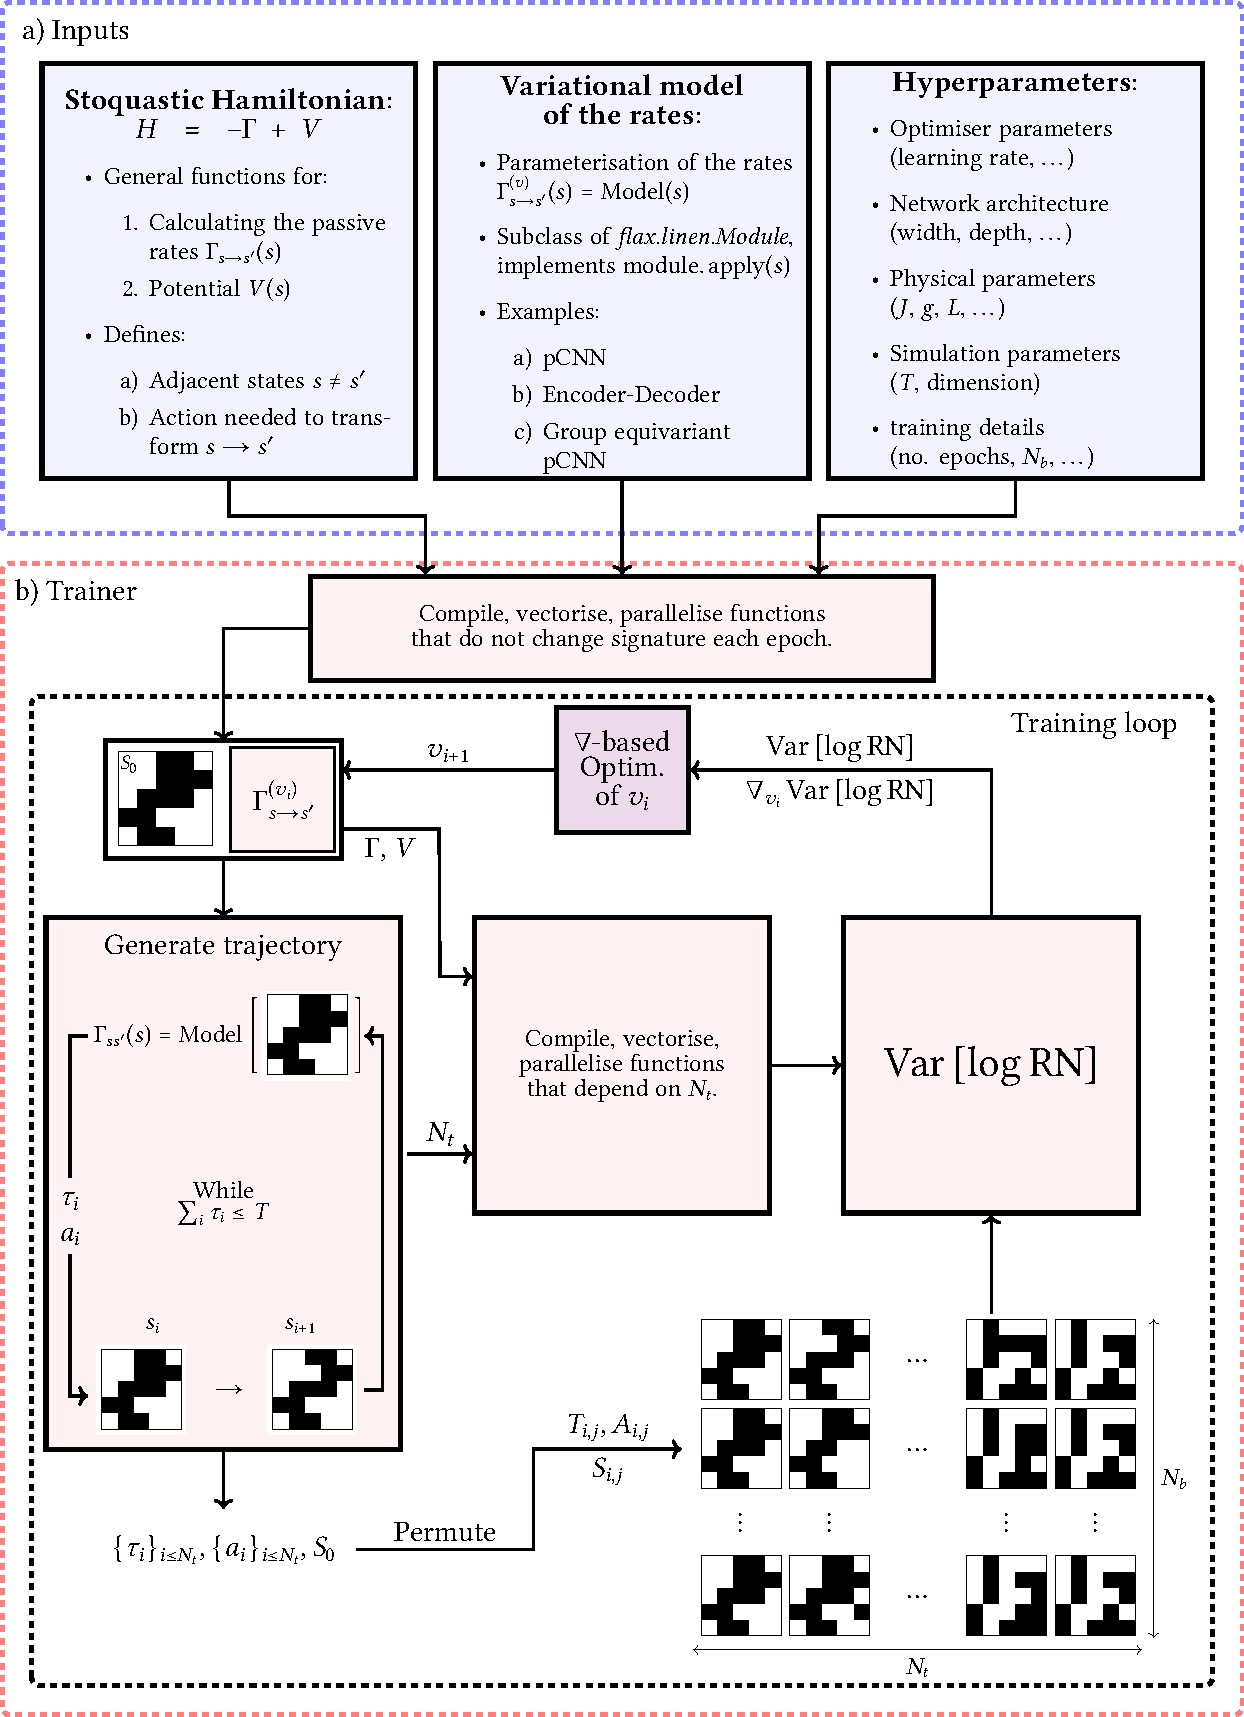
\includegraphics[width=\linewidth]{Chapter4/Figs/Vector/qsampl1}
\end{figure}
\begin{figure}[t]
	\ContinuedFloat
	\centering
	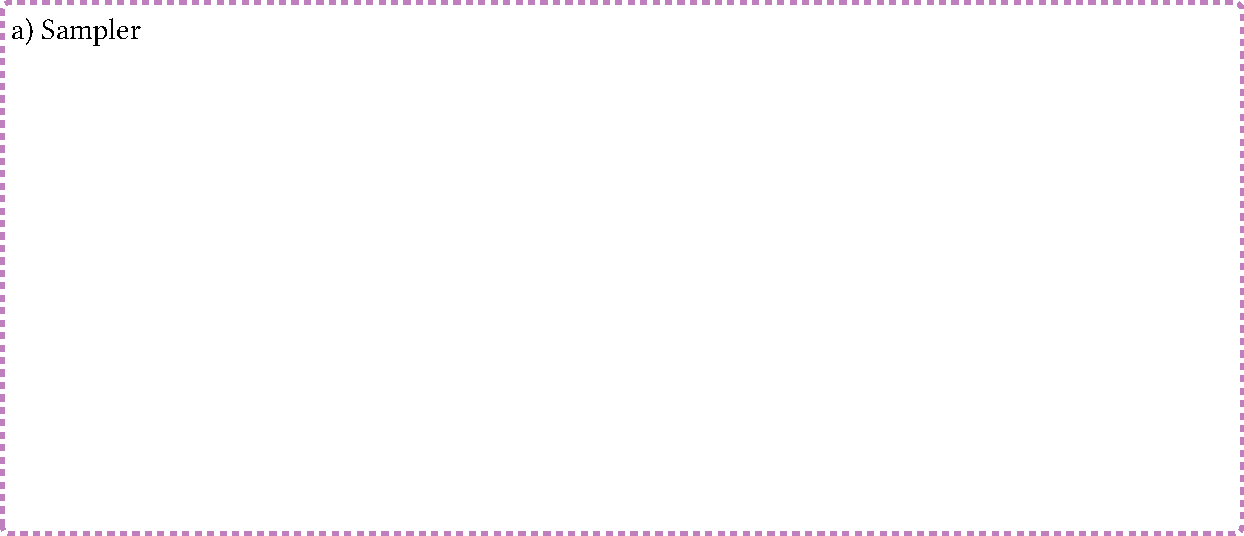
\includegraphics[width=\linewidth]{Chapter4/Figs/Vector/qsampl2}
	\caption[Implementation details]{\textbf{Implementation details}}
	\label{fig:qsampl}
\end{figure}

\nomenclature[z-gCNN]{G-CNN}{Group Convolutional Neural Network}